%% ============================================================
%%  CSE344 – System Programming | Homework #4 Report
%%  Halit Batuhan ASLAN | 220104004003 | Spring 2026
%% ============================================================
\documentclass[12pt,a4paper]{article}

% ── Packages ──────────────────────────────────────────────────
\usepackage[T1]{fontenc}
\usepackage[utf8]{inputenc}
\usepackage[english]{babel}
\usepackage{geometry}
\geometry{a4paper, top=2.5cm, bottom=2.5cm, left=2.5cm, right=2.5cm}

\usepackage{parskip}
\usepackage{setspace}
\onehalfspacing

\usepackage{graphicx}
\usepackage{float}
\usepackage{caption}
\usepackage{subcaption}

\usepackage{booktabs}
\usepackage{array}
\usepackage{longtable}
\usepackage{tabularx}
\usepackage{multirow}
\usepackage{colortbl}
\usepackage{xcolor}

\usepackage{listings}
\usepackage{fancyvrb}

\usepackage{hyperref}
\hypersetup{
    colorlinks=true,
    linkcolor=blue!60!black,
    urlcolor=blue!60!black,
    citecolor=blue!60!black,
    pdftitle={CSE344 HW4 Report},
    pdfauthor={Halit Batuhan ASLAN}
}

\usepackage{enumitem}
\usepackage{fancyhdr}
\usepackage{titlesec}
\usepackage{mdframed}
\usepackage{tcolorbox}
\tcbuselibrary{skins,breakable}
\usepackage{tikz}
\usetikzlibrary{shapes.geometric, arrows.meta, positioning, fit, backgrounds, decorations.pathreplacing}
\usepackage{forest}
\usepackage{amsmath}
\usepackage{amssymb}
\usepackage{pifont}

% ── Colors ────────────────────────────────────────────────────
\definecolor{codeblue}{RGB}{0,80,160}
\definecolor{codegray}{RGB}{245,245,245}
\definecolor{codegreen}{RGB}{0,128,0}
\definecolor{codepurple}{RGB}{128,0,128}
\definecolor{headerblue}{RGB}{28,78,148}
\definecolor{lightblue}{RGB}{219,234,254}
\definecolor{lightgreen}{RGB}{220,252,231}
\definecolor{lightyellow}{RGB}{254,249,195}
\definecolor{lightred}{RGB}{254,226,226}
\definecolor{darkgray}{RGB}{55,65,81}
\definecolor{borderblue}{RGB}{147,197,253}
\definecolor{accentorange}{RGB}{234,88,12}

% ── Code listings ─────────────────────────────────────────────
\lstdefinestyle{cstyle}{
    language=C,
    backgroundcolor=\color{codegray},
    basicstyle=\ttfamily\footnotesize,
    keywordstyle=\color{codeblue}\bfseries,
    commentstyle=\color{codegreen}\itshape,
    stringstyle=\color{codepurple},
    numbers=left,
    numberstyle=\tiny\color{gray},
    numbersep=6pt,
    stepnumber=1,
    frame=single,
    framerule=0.5pt,
    rulecolor=\color{gray!40},
    breaklines=true,
    breakatwhitespace=true,
    tabsize=4,
    showstringspaces=false,
    captionpos=b,
    xleftmargin=12pt,
    xrightmargin=4pt,
}
\lstset{style=cstyle}

% ── Custom boxes ──────────────────────────────────────────────
\tcbset{
    warningbox/.style={
        enhanced, breakable,
        colback=lightyellow, colframe=yellow!60!black,
        fonttitle=\bfseries, title=\ding{78}~Warning,
        left=4pt, right=4pt, top=4pt, bottom=4pt
    },
    infobox/.style={
        enhanced, breakable,
        colback=lightblue, colframe=headerblue,
        fonttitle=\bfseries, title=\ding{72}~Note,
        left=4pt, right=4pt, top=4pt, bottom=4pt
    },
    okbox/.style={
        enhanced, breakable,
        colback=lightgreen, colframe=green!50!black,
        fonttitle=\bfseries, title=\ding{52}~Correct,
        left=4pt, right=4pt, top=4pt, bottom=4pt
    }
}

% ── Header / Footer ───────────────────────────────────────────
\pagestyle{fancy}
\fancyhf{}
\fancyhead[L]{\small\color{darkgray} CSE344 – System Programming $\mid$ Homework \#4}
\fancyhead[R]{\small\color{darkgray} Halit Batuhan ASLAN}
\fancyfoot[C]{\small\thepage}
\renewcommand{\headrulewidth}{0.4pt}
\renewcommand{\footrulewidth}{0pt}

% ── Section formatting ────────────────────────────────────────
\titleformat{\section}{\large\bfseries\color{headerblue}}{{\thesection}}{0.8em}{}[\color{headerblue}\titlerule]
\titleformat{\subsection}{\normalsize\bfseries\color{darkgray}}{{\thesubsection}}{0.6em}{}
\titleformat{\subsubsection}{\normalsize\itshape\color{darkgray}}{{\thesubsubsection}}{0.5em}{}

% ── Helpers ───────────────────────────────────────────────────
\newcommand{\code}[1]{\texttt{\small #1}}
\newcommand{\ck}{\ding{52}}   % check
\newcommand{\cx}{\ding{56}}   % cross

% ══════════════════════════════════════════════════════════════
\begin{document}

% ── Title Page ────────────────────────────────────────────────
\begin{titlepage}
\centering
\vspace*{1.5cm}

{\color{headerblue}\rule{\linewidth}{2pt}}
\vspace{0.5cm}

{\LARGE\bfseries CSE344 -- System Programming}\\[0.4cm]
{\Large Homework \#4 Report}\\[0.2cm]
{\large Multi-Process \& Multi-Threaded Concurrent Log Analysis Pipeline}

\vspace{0.4cm}
{\color{headerblue}\rule{\linewidth}{1pt}}
\vspace{1.2cm}

\begin{tabular}{rl}
\textbf{Name \& Surname:} & Halit Batuhan ASLAN \\[4pt]
\textbf{Student ID:}       & 220104004003 \\[4pt]
\textbf{Course:}           & CSE344 -- System Programming \\[4pt]
\textbf{Semester:}         & Spring 2026 \\[4pt]
\textbf{Platform:}         & Debian 12 (64-bit) -- VirtualBox \\[4pt]
\textbf{Language:}         & C (POSIX-compliant) \\
\end{tabular}

\vfill
{\small\color{darkgray} \today}
\end{titlepage}

% ── Table of Contents ─────────────────────────────────────────
\tableofcontents
\newpage

% ══════════════════════════════════════════════════════════════
\section{Introduction}
% ══════════════════════════════════════════════════════════════

\subsection{Problem Description}

This homework requires the design and implementation of a \textbf{Concurrent Log Analysis Pipeline} in C using both multi-process and multi-threaded paradigms simultaneously. The system reads multiple log files concurrently, classifies entries by severity level (ERROR, WARN, INFO, DEBUG), performs weighted keyword scoring with overlapping match detection, identifies high-priority sources, and produces structured output in text and binary formats.

The system must correctly employ every synchronization primitive taught in the course: \code{pthread\_mutex\_t}, \code{pthread\_cond\_t}, \code{pthread\_cond\_timedwait}, \code{pthread\_barrier\_t}, \code{pthread\_key\_t} (TLS), \code{sem\_t}, \code{volatile sig\_atomic\_t}, and \code{sigaction}.

\subsection{Main Challenges}

\begin{enumerate}[leftmargin=*, label=\textbf{\arabic*.}]
    \item \textbf{Cross-process shared memory:} Four separate \code{mmap(MAP\_SHARED|MAP\_ANONYMOUS)} regions must be initialized with \code{PTHREAD\_PROCESS\_SHARED} attributes before any \code{fork()}, so all child processes can use the same synchronization primitives.
    \item \textbf{EOF propagation chain:} With $N$ reader processes each sending 4 EOF markers (one per level) to Region~A, the Dispatcher must correctly count and forward them to the appropriate Region~B buffers.
    \item \textbf{TLS flush ordering:} Worker threads accumulate keyword scores in thread-local storage. The flush to Region~C must happen in the destructor (at thread exit), not at the barrier --- a subtle ordering constraint that was specifically tested.
    \item \textbf{Concurrent Region~D consumption:} The Aggregator must drain Region~D while simultaneously waiting for Region~C semaphores, requiring a dedicated drain thread to avoid deadlock.
    \item \textbf{Correct byte-range splitting:} Reader threads divide a file into byte ranges; a range boundary that falls mid-line must be resolved by having the next thread skip to the next newline.
\end{enumerate}

\subsection{Approach}

The implementation follows an incremental strategy: the internal buffer (Reader-private) was implemented and tested first, followed by Region~A, then Region~B, and finally TLS/Barrier/Aggregator. Each stage was validated with a single-threaded, single-process configuration before introducing concurrency.

% ══════════════════════════════════════════════════════════════
\section{System Architecture}
% ══════════════════════════════════════════════════════════════

\subsection{Process and Thread Hierarchy}

\begin{table}[H]
\centering
\caption{All process and thread types in the system}
\renewcommand{\arraystretch}{1.25}
\begin{tabularx}{\linewidth}{lllX}
\toprule
\textbf{Component} & \textbf{Type} & \textbf{Count} & \textbf{Responsibility} \\
\midrule
Parent / Coordinator & Process & 1 & Fork chain, SHM init, waitpid, final summary \\
Watchdog & pthread (in Parent) & 1 & Pipe \code{select()}, stderr progress every 3s \\
Reader & Process & $N$ (one per log file) & File reading, internal buffer, Region~A push \\
Reader Thread & pthread (in Reader) & $T$ per Reader & Byte-range reading $\to$ internal buffer \\
Parser Thread & pthread (in Reader) & 1 per Reader & Internal buffer $\to$ Region~A \\
Dispatcher & Process & 1 & Region~A $\to$ Region~B + D routing \\
Analyzer ERROR & Process & 1 & Region~B[0] $\to$ Region~C \\
Analyzer WARN & Process & 1 & Region~B[1] $\to$ Region~C \\
Analyzer INFO & Process & 1 & Region~B[2] $\to$ Region~C \\
Analyzer DEBUG & Process & 1 & Region~B[3] $\to$ Region~C \\
Worker Thread & pthread (in Analyzer) & $W$ per Analyzer & Consume, TLS accumulate, barrier \\
Aggregator & Process & 1 & Region~C + D $\to$ output files \\
\bottomrule
\end{tabularx}
\end{table}

Total \code{fork()} calls: $N + 1 + 4 + 1 = N + 6$ child processes.

Total \code{pthread\_create()} calls: $1$ (Watchdog) $+ N \times (T+1)$ (Readers) $+ 4 \times W$ (Analyzers).

\subsection{Architecture Diagram}

\begin{figure}[H]
\centering
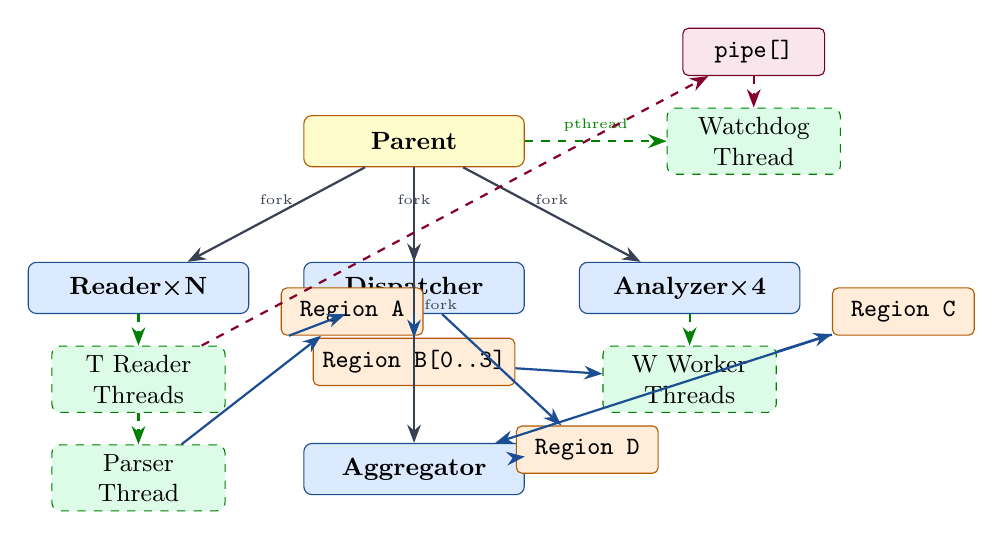
\begin{tikzpicture}[
    node distance=0.5cm and 0.8cm,
    proc/.style={rectangle, draw=headerblue, fill=lightblue, rounded corners=3pt,
                 minimum width=2.8cm, minimum height=0.65cm, font=\small\bfseries, align=center},
    thread/.style={rectangle, draw=green!50!black, fill=lightgreen, rounded corners=3pt,
                   minimum width=2.2cm, minimum height=0.55cm, font=\small, align=center,
                   dashed},
    shm/.style={rectangle, draw=orange!70!black, fill=orange!15, rounded corners=2pt,
                minimum width=1.8cm, minimum height=0.6cm, font=\small\ttfamily, align=center},
    arr/.style={-Stealth, thick, color=darkgray},
    darr/.style={-Stealth, thick, color=green!50!black, dashed}
]

% Parent
\node[proc, fill=yellow!20, draw=orange!70!black] (parent) {Parent};

% Watchdog
\node[thread, right=1.8cm of parent] (wdog) {Watchdog\\Thread};

% Reader
\node[proc, below=1.2cm of parent, xshift=-3.5cm] (reader) {Reader×N};
\node[thread, below=0.4cm of reader] (rthread) {T Reader\\Threads};
\node[thread, below=0.4cm of rthread] (pthread) {Parser\\Thread};

% Dispatcher
\node[proc, below=1.2cm of parent] (disp) {Dispatcher};

% Analyzers
\node[proc, below=1.2cm of parent, xshift=3.5cm] (anal) {Analyzer×4};
\node[thread, below=0.4cm of anal] (wthread) {W Worker\\Threads};

% Aggregator
\node[proc, below=3.5cm of parent] (agg) {Aggregator};

% SHM Regions
\node[shm, right=0.4cm of reader, yshift=-0.3cm] (regA) {Region A};
\node[shm, below=0.3cm of disp] (regB) {Region B[0..3]};
\node[shm, right=0.4cm of anal, yshift=-0.3cm] (regC) {Region C};
\node[shm, below=0.5cm of regB, xshift=2.2cm] (regD) {Region D};

% Pipe
\node[shm, draw=purple!60!black, fill=purple!10, above=0.4cm of wdog] (pipe) {pipe[]};

% Arrows
\draw[arr] (parent) -- node[above, font=\tiny]{fork} (reader);
\draw[arr] (parent) -- node[above, font=\tiny]{fork} (disp);
\draw[arr] (parent) -- node[above, font=\tiny]{fork} (anal);
\draw[arr] (parent) -- node[right, font=\tiny]{fork} (agg);
\draw[darr] (parent) -- node[above, font=\tiny]{pthread} (wdog);

\draw[darr] (reader) -- (rthread);
\draw[darr] (rthread) -- (pthread);
\draw[darr] (anal) -- (wthread);

\draw[arr, color=headerblue] (pthread) -- (regA);
\draw[arr, color=headerblue] (regA) -- (disp);
\draw[arr, color=headerblue] (disp) -- (regB);
\draw[arr, color=headerblue] (disp) -- (regD);
\draw[arr, color=headerblue] (regB) -- (wthread);
\draw[arr, color=headerblue] (wthread) -- (regC);
\draw[arr, color=headerblue] (regC) -- (agg);
\draw[arr, color=headerblue] (regD) -- (agg);

\draw[arr, color=purple!70!black, dashed] (rthread) -- (pipe);
\draw[arr, color=purple!70!black, dashed] (pipe) -- (wdog);

\end{tikzpicture}
\caption{System architecture: processes, threads, and shared memory data flow}
\label{fig:arch}
\end{figure}

% ══════════════════════════════════════════════════════════════
\section{Shared Memory Layout}
% ══════════════════════════════════════════════════════════════

\subsection{Overview of Four Regions}

All regions are allocated with \code{mmap(MAP\_SHARED|MAP\_ANONYMOUS)} in the parent \textbf{before} any \code{fork()} call. Each region uses flexible arrays (\code{buf[]}) so the circular buffer is contiguous with the header struct in memory.

\begin{table}[H]
\centering
\caption{Shared memory regions}
\renewcommand{\arraystretch}{1.3}
\begin{tabularx}{\linewidth}{llXll}
\toprule
\textbf{Region} & \textbf{Struct} & \textbf{Size Formula} & \textbf{Writers} & \textbf{Readers} \\
\midrule
A & \code{shm\_region\_a\_t} & \code{sizeof(hdr) + cap\_A × sizeof(entry)} & Reader parsers & Dispatcher \\
B×4 & \code{shm\_region\_b\_t} & \code{sizeof(hdr) + cap\_B × sizeof(entry)} & Dispatcher only & Analyzer workers \\
C & \code{shm\_region\_c\_t} & \code{sizeof(shm\_region\_c\_t)} (fixed) & Analyzer reporter & Aggregator \\
D & \code{shm\_region\_d\_t} & \code{sizeof(hdr) + cap\_D × sizeof(entry)} & Dispatcher only & Aggregator drain thread \\
\bottomrule
\end{tabularx}
\end{table}

\subsection{Struct Definitions}

\subsubsection{log\_entry\_t --- Basic Data Unit}

\begin{lstlisting}[caption={log\_entry\_t: the fundamental data unit passed between all regions}]
typedef struct {
    char timestamp[20];   /* "YYYY-MM-DD HH:MM:SS\0" */
    int  level;           /* 0=ERROR, 1=WARN, 2=INFO, 3=DEBUG */
    char source[64];      /* alphanumeric source identifier     */
    char message[1024];   /* log message body                   */
    int  is_eof;          /* 1 = EOF sentinel, not a real entry */
} log_entry_t;
\end{lstlisting}

\subsubsection{level\_result\_t --- Region~C Result per Level}

\begin{lstlisting}[caption={level\_result\_t: result written by each Analyzer to Region C}]
typedef struct {
    char   level[8];                         /* "ERROR", "WARN", ... */
    long   total_entries;
    double total_weighted_score;
    double per_keyword_score[MAX_KEYWORDS];  /* one per keyword       */
    double per_thread_score[MAX_WORKERS];    /* one per worker thread */
    char   top_source[3][MAX_SOURCE_LEN];   /* top-3 sources by hits */
    long   top_source_hits[3];
    int    ready;                            /* 1 when Analyzer done  */
} level_result_t;
\end{lstlisting}

\subsubsection{Region~A --- shm\_region\_a\_t}

\begin{lstlisting}[caption={Region A: dispatcher input queue (all reader parsers write, dispatcher reads)}]
typedef struct {
    pthread_mutex_t input_mutex;          /* PTHREAD_PROCESS_SHARED */
    pthread_cond_t  not_full_a;           /* PTHREAD_PROCESS_SHARED */
    pthread_cond_t  not_empty_a;          /* PTHREAD_PROCESS_SHARED */
    int  eof_count_per_level[LEVEL_COUNT];/* incremented by parsers  */
    int  total_readers;                   /* set by parent before fork*/
    int  head, tail, count, capacity;
    log_entry_t buf[];                    /* flexible array          */
} shm_region_a_t;
\end{lstlisting}

\textbf{Which primitive protects which field:}
\code{input\_mutex} protects \code{head}, \code{tail}, \code{count}, \code{buf[]}, and \code{eof\_count\_per\_level[]}.
\code{not\_full\_a} is signaled when an entry is consumed (pop).
\code{not\_empty\_a} is broadcast when an entry is added (push) or an EOF is counted.

\subsubsection{Region~B --- shm\_region\_b\_t (×4)}

\begin{lstlisting}[caption={Region B: per-level analysis buffer (Dispatcher writes, Analyzer workers read)}]
typedef struct {
    pthread_mutex_t level_mutex;   /* PTHREAD_PROCESS_SHARED */
    pthread_cond_t  not_full_b;    /* PTHREAD_PROCESS_SHARED */
    pthread_cond_t  not_empty_b;   /* PTHREAD_PROCESS_SHARED */
    int  eof_posted;               /* 1 when Dispatcher done for this level */
    int  head, tail, count, capacity;
    log_entry_t buf[];
} shm_region_b_t;
\end{lstlisting}

\textbf{Key design:} The Dispatcher is the \emph{sole writer} to Region~B and Region~D. This single-writer constraint eliminates write-write races and simplifies synchronization: Analyzer worker threads only need to synchronize among themselves (readers) using \code{level\_mutex}.

\subsubsection{Region~C --- shm\_region\_c\_t}

\begin{lstlisting}[caption={Region C: results area; fixed size, no circular buffer}]
typedef struct {
    pthread_mutex_t result_mutex;          /* PTHREAD_PROCESS_SHARED */
    pthread_cond_t  result_cond;           /* PTHREAD_PROCESS_SHARED */
    sem_t           level_sems[LEVEL_COUNT];/* process-shared unnamed  */
    level_result_t  results[LEVEL_COUNT];  /* one per level           */
} shm_region_c_t;
\end{lstlisting}

\textbf{Primitive roles:} \code{result\_mutex} protects \code{results[]} during writes from the reporting thread and TLS destructor. \code{level\_sems[i]} is posted by the reporting thread of Analyzer~$i$ and waited on (with timeout) by the Aggregator.

\subsubsection{Region~D --- shm\_region\_d\_t}

\begin{lstlisting}[caption={Region D: high-priority buffer for filter-matching entries}]
typedef struct {
    pthread_mutex_t priority_mutex;   /* PTHREAD_PROCESS_SHARED */
    pthread_cond_t  not_full_d;       /* PTHREAD_PROCESS_SHARED */
    pthread_cond_t  not_empty_d;      /* PTHREAD_PROCESS_SHARED */
    int  dispatcher_done;             /* 1 when Dispatcher exits */
    int  head, tail, count, capacity;
    log_entry_t buf[];
} shm_region_d_t;
\end{lstlisting}

% ══════════════════════════════════════════════════════════════
\section{Lock Ordering and Deadlock Prevention}
% ══════════════════════════════════════════════════════════════

\subsection{Global Lock Acquisition Order}

A strict global ordering is defined and enforced throughout the codebase:

\begin{table}[H]
\centering
\caption{Mandatory lock acquisition order}
\renewcommand{\arraystretch}{1.3}
\begin{tabular}{clll}
\toprule
\textbf{Priority} & \textbf{Mutex} & \textbf{Location} & \textbf{Rule} \\
\midrule
1 (first) & \code{input\_mutex}      & Region A & May not be held while acquiring others \\
2          & \code{level\_mutex[i]}   & Region B & Acquire only after releasing Region~A mutex \\
3          & \code{result\_mutex}     & Region C & Acquire only after releasing Region~B mutex \\
4 (last)  & \code{priority\_mutex}   & Region D & Acquire only after releasing all others \\
\bottomrule
\end{tabular}
\end{table}

\subsection{Deadlock Freedom Proof}

\textbf{Claim:} No circular wait can occur.

\textbf{Proof sketch:} Label the four mutexes $M_1$ (Region~A), $M_2$ (Region~B), $M_3$ (Region~C), $M_4$ (Region~D) such that $i < j \Rightarrow M_i$ has higher priority. By the acquisition order rule, any thread that holds $M_i$ may never subsequently request $M_j$ where $j < i$. Therefore the \emph{wait-for} graph is a DAG (directed acyclic graph) with edges only from lower-index to higher-index nodes. A DAG has no cycle, so deadlock is impossible. \hfill$\square$

\subsection{Additional Locking Rules}

\begin{itemize}[leftmargin=*]
    \item No blocking I/O (\code{read}, \code{write}, \code{printf}) is called while holding any mutex.
    \item In practice, each function acquires at most one mutex at a time, so the ordering is trivially respected. No function holds two region mutexes simultaneously.
\end{itemize}

% ══════════════════════════════════════════════════════════════
\section{Thread Lifecycle}
% ══════════════════════════════════════════════════════════════

\subsection{Reader Thread Lifecycle}

\begin{enumerate}[leftmargin=*, label=\textbf{Step \arabic*.}]
    \item \textbf{Creation:} \code{pthread\_create} from \code{reader\_process\_main()}. Arguments include byte range [\code{start\_byte}, \code{end\_byte}), file path, pipe write FD, and a pointer to the shared \code{internal\_buf\_t}.
    \item \textbf{File open \& seek:} \code{fopen} + \code{fseek(start\_byte)}. If \code{start\_byte > 0}, the first partial line is skipped with one \code{fgets} call to avoid double-processing.
    \item \textbf{Read loop:} \code{fgets} reads lines. If \code{ftell() > end\_byte}, the thread stops (boundary condition). Each line is passed to \code{parse\_log\_line()}.
    \item \textbf{Parse:} Valid entries are pushed to \code{internal\_buf\_t} via \code{ibuf\_push()} (mutex + condvar, blocks if buffer is full).
    \item \textbf{Heartbeat:} Every 50 lines, \code{write(pipe\_write\_fd, "[R\%d] \%ld lines processed\textbackslash n")} is called.
    \item \textbf{Termination:} After the read loop, \code{finished\_producers++} is incremented under the internal buffer mutex, and \code{pthread\_cond\_broadcast} wakes the parser thread.
    \item \textbf{Exit:} \code{return NULL}.
\end{enumerate}

\subsection{Worker Thread Lifecycle}

\begin{enumerate}[leftmargin=*, label=\textbf{Step \arabic*.}]
    \item \textbf{Creation:} \code{pthread\_create} from \code{analyzer\_process\_main()}.
    \item \textbf{TID registration:} \code{pid\_t my\_tid = (pid\_t)syscall(SYS\_gettid)} is called and stored in \code{g\_tids[]} under \code{g\_tid\_mu}.
    \item \textbf{TLS initialization:} \code{calloc(n\_keywords, sizeof(double))} allocates the score array. \code{pthread\_setspecific(g\_tls\_key, tls)} registers it.
    \item \textbf{Consume loop:} \code{shm\_b\_pop()} retrieves entries from Region~B (blocks on \code{not\_empty\_b} condvar, returns 0 when \code{eof\_posted=1} and buffer empty).
    \item \textbf{Score accumulation:} For each entry, \code{count\_overlapping(message, keyword[k])} is called and the result multiplied by \code{LEVEL\_WEIGHTS[level\_idx]}. Score is added to \code{tls[k]} \textbf{without any mutex} --- this is the key TLS benefit.
    \item \textbf{Source tracking:} \code{srcmap\_add(\&local\_src, entry.source)} maintains a local per-source hit count.
    \item \textbf{Global merge:} After the consume loop, global statistics (\code{g\_total\_entries}, \code{g\_total\_weighted}, \code{g\_src\_map}) are updated under \code{g\_agg\_mu}.
    \item \textbf{Barrier:} \code{pthread\_barrier\_wait(\&g\_barrier)} --- all $W$ workers synchronize here. No TLS flush happens at this point.
    \item \textbf{Reporter selection:} After the barrier, the minimum TID among \code{g\_tids[0..W-1]} is computed under \code{g\_tid\_mu}. The thread with \code{my\_tid == min\_tid} becomes the reporting thread.
    \item \textbf{Reporting (reporting thread only):} Under \code{result\_mutex}: writes \code{total\_entries}, \code{total\_weighted\_score}, top-3 sources to \code{region\_c->results[level\_idx]}; sets \code{ready=1}; calls \code{sem\_post(\&level\_sems[level\_idx])}.
    \item \textbf{Exit:} \code{return NULL} triggers the TLS destructor.
    \item \textbf{TLS destructor (\code{tls\_destructor}):} Acquires \code{result\_mutex}; adds \code{tls[k]} to \code{per\_keyword\_score[k]} and records \code{per\_thread\_score[idx]}; releases mutex; calls \code{free(tls)}.
\end{enumerate}

\begin{tcolorbox}[warningbox]
The critical ordering is: \textbf{barrier\_wait()} $\to$ \textbf{reporter writes Region~C} $\to$ \textbf{return NULL} $\to$ \textbf{destructor flushes TLS}. Flushing TLS at the barrier instead of at thread exit is a common mistake --- the destructor cannot run until the thread exits, so per\_keyword\_score values would be missing from Region~C if flushed too early.
\end{tcolorbox}

% ══════════════════════════════════════════════════════════════
\section{TLS Design}
% ══════════════════════════════════════════════════════════════

\subsection{Purpose}

Thread-Local Storage allows each worker thread to accumulate per-keyword weighted scores \emph{without holding any mutex}. The accumulation is entirely private to the thread. Only when the thread exits does the destructor flush the data to the shared \code{level\_result\_t} in Region~C under \code{result\_mutex}.

\subsection{Usage Pattern}

\begin{lstlisting}[caption={TLS setup, usage, and destruction in Analyzer}]
/* === Analyzer main (before pthread_create) === */
pthread_key_t g_tls_key;
pthread_key_create(&g_tls_key, tls_destructor);  /* register destructor */

/* === Worker thread start === */
double* tls = calloc(n_keywords, sizeof(double));
pthread_setspecific(g_tls_key, tls);              /* bind to this thread */

/* === Worker thread work loop (NO mutex) === */
tls[k] += count_overlapping(msg, kw[k]) * weight;

/* === Worker thread: return NULL ==> tls_destructor called === */

/* === tls_destructor === */
void tls_destructor(void* val) {
    double* scores = (double*)val;
    int idx = __sync_fetch_and_add(&g_dest_idx, 1);
    pthread_mutex_lock(&region_c->result_mutex);
    for (int k = 0; k < n_keywords; k++)
        region_c->results[level].per_keyword_score[k] += scores[k];
    region_c->results[level].per_thread_score[idx] = sum(scores);
    pthread_mutex_unlock(&region_c->result_mutex);
    free(scores);
}
\end{lstlisting}

\subsection{Why Flush in Destructor, Not at Barrier?}

The \code{pthread\_barrier\_wait()} call synchronizes thread \emph{execution}, not thread \emph{exit}. After the barrier, threads still execute (the reporter writes to Region~C). The destructor is invoked by the pthreads runtime only when the thread fully exits (\code{return NULL} completes). If the flush were attempted at the barrier, the destructor would \emph{still run later} at thread exit and double-count the scores (or write over already-correct values). The correct design is to let the destructor be the single, authoritative flush point.

% ══════════════════════════════════════════════════════════════
\section{Dispatcher Logic}
% ══════════════════════════════════════════════════════════════

\subsection{EOF Marker Management}

With $N$ Reader processes and 4 severity levels, the system produces $4N$ EOF markers in Region~A (each parser thread sends one EOF per level). The Dispatcher tracks them with:

\begin{lstlisting}[caption={Dispatcher EOF tracking}]
int eof_received[LEVEL_COUNT]  = {0};
int eof_forwarded[LEVEL_COUNT] = {0};

/* Inside the main loop: */
if (entry.is_eof) {
    eof_received[entry.level]++;
    /* When all N readers have sent EOF for this level: */
    if (eof_received[entry.level] >= n_readers && !eof_forwarded[entry.level]) {
        signal_eof_to_b(region_b[entry.level]);  /* eof_posted=1 + broadcast */
        eof_forwarded[entry.level] = 1;
    }
    /* If all 4 levels forwarded: break main loop */
    if (all_4_forwarded) break;
    continue;
}
\end{lstlisting}

The key invariant is: Region~B[level] only receives its \code{eof\_posted=1} signal after \emph{all $N$ readers} have confirmed they have no more entries at that level. This prevents premature termination in Analyzer worker threads.

\subsection{Priority Source Filtering}

For each real (non-EOF) entry, the Dispatcher checks whether \code{entry.source} appears in the priority list loaded at startup. If it matches, the entry is pushed to \emph{both} Region~B (for keyword analysis) and Region~D (for high-priority scoring by the Aggregator).

\subsection{Single-Writer Design}

The Dispatcher is the \textbf{only process that writes to Region~B and Region~D}. This simplifies synchronization significantly: the consumer side (Analyzer workers for B, Aggregator drain thread for D) only needs to protect concurrent reads among themselves --- no write-write race is possible.

% ══════════════════════════════════════════════════════════════
\section{Termination Chain}
% ══════════════════════════════════════════════════════════════

\subsection{Normal Termination}

\begin{enumerate}[leftmargin=*, label=\textbf{Step \arabic*.}]
    \item \textbf{Reader Processes ($\times N$):} All reader threads finish their byte ranges $\to$ parser thread drains the internal buffer $\to$ parser sends 4 EOF markers to Region~A $\to$ \code{exit(0)}.
    \item \textbf{Dispatcher:} Receives $4N$ EOF markers from Region~A $\to$ forwards 4 level-specific EOFs to Region~B $\to$ sets \code{dispatcher\_done=1} and broadcasts Region~D condvar $\to$ \code{exit(0)}.
    \item \textbf{Analyzer Processes ($\times 4$):} Worker threads drain Region~B (stop when \code{eof\_posted=1} and buffer empty) $\to$ \code{pthread\_barrier\_wait} $\to$ reporting thread writes Region~C and calls \code{sem\_post} $\to$ all workers \code{return NULL} triggering TLS destructors $\to$ \code{exit(0)}.
    \item \textbf{Aggregator:} \code{sem\_timedwait} on all 4 level semaphores completes $\to$ drain thread joins $\to$ results sorted, text and binary files written $\to$ \code{exit(0)}.
    \item \textbf{Parent:} \code{waitpid} loop collects all $N+6$ children $\to$ \code{shutdown\_watchdog=1} $\to$ \code{pthread\_join(watchdog)} $\to$ final summary printed to stdout $\to$ \code{shm\_destroy\_*()} releases all \code{mmap} regions $\to$ \code{return 0}.
\end{enumerate}

\subsection{SIGINT (Ctrl+C) Handling}

\begin{lstlisting}[caption={SIGINT handler and cleanup sequence}]
/* Handler - only async-signal-safe operations: */
static void sigint_handler(int sig) {
    (void)sig;
    sigint_received = 1;          /* volatile sig_atomic_t */
}

/* Parent main loop detects the flag: */
if (sigint_received) {
    for (int i = 0; i < n_children; i++)
        kill(child_pids[i], SIGTERM);          /* 1. SIGTERM to all children */

    time_t deadline = time(NULL) + 5;
    while (children_alive > 0 && time(NULL) < deadline) {
        pid_t p = waitpid(-1, &st, WNOHANG);  /* 2. Non-blocking wait */
        if (p > 0) children_alive--;
        else usleep(20000);
    }
    shutdown_watchdog = 1;
    pthread_join(watchdog_tid, NULL);          /* 3. Stop Watchdog     */
    cleanup_and_exit(1);                       /* 4. munmap + _exit(1) */
}
\end{lstlisting}

\begin{tcolorbox}[infobox]
\code{printf}, \code{malloc}, and \code{free} are \textbf{never called} inside the SIGINT handler. Only \code{sigint\_received = 1} (a simple flag write) is performed, which is guaranteed to be async-signal-safe.
\end{tcolorbox}

% ══════════════════════════════════════════════════════════════
\section{Keyword Weighted Scoring Algorithm}
% ══════════════════════════════════════════════════════════════

\subsection{Overlapping Substring Search}

The standard \code{strstr()} function advances past the end of each match, missing overlapping occurrences. A sliding-window approach is used instead:

\begin{lstlisting}[caption={Overlapping substring count (sliding window)}]
int count_overlapping(const char* text, const char* keyword) {
    int count = 0;
    int klen  = (int)strlen(keyword);
    int tlen  = (int)strlen(text);
    if (klen == 0 || klen > tlen) return 0;
    for (int i = 0; i <= tlen - klen; i++)
        if (memcmp(text + i, keyword, klen) == 0) count++;
    return count;
}
\end{lstlisting}

\textbf{Example:} The string \texttt{"errorer"} contains \texttt{"error"} at index 0 and index 3, giving a count of 2. \code{strstr} would only find the first match.

\subsection{Weighted Score Formula}

\[
\text{score}(e, k) = \text{count\_overlapping}(e.\text{message},\, k) \times w_{\text{level}(e)}
\]

where level weights are:

\begin{center}
\begin{tabular}{lc}
\toprule
\textbf{Level} & \textbf{Weight} \\
\midrule
ERROR & 4 \\
WARN  & 3 \\
INFO  & 2 \\
DEBUG & 1 \\
\bottomrule
\end{tabular}
\end{center}

The total weighted score for level $\ell$ and keyword $k$ is:
\[
S(\ell,k) = \sum_{e\,:\,e.\text{level}=\ell} \text{score}(e, k)
\]

These per-keyword, per-level scores are accumulated in TLS arrays and flushed to \code{per\_keyword\_score[k]} in Region~C by the TLS destructor.

% ══════════════════════════════════════════════════════════════
\section{Synchronization Primitives Summary}
% ══════════════════════════════════════════════════════════════

\begin{longtable}{p{4.2cm}p{2.8cm}p{1.6cm}p{5cm}}
\caption{All synchronization primitives used in the system} \\
\toprule
\textbf{Primitive} & \textbf{Location} & \textbf{Attr.} & \textbf{Purpose} \\
\midrule
\endfirsthead
\toprule
\textbf{Primitive} & \textbf{Location} & \textbf{Attr.} & \textbf{Purpose} \\
\midrule
\endhead
\bottomrule
\endfoot
\code{pthread\_mutex\_t input\_mutex} & Region A & PROC\_SH & Protect all A fields from concurrent reader parsers and Dispatcher \\[2pt]
\code{pthread\_cond\_t not\_full\_a} & Region A & PROC\_SH & Block parser threads when buffer full \\[2pt]
\code{pthread\_cond\_t not\_empty\_a} & Region A & PROC\_SH & Block Dispatcher when buffer empty \\[2pt]
\code{pthread\_mutex\_t level\_mutex[i]} & Region B ×4 & PROC\_SH & Protect B[i] from concurrent Analyzer workers \\[2pt]
\code{pthread\_cond\_t not\_full\_b[i]} & Region B ×4 & PROC\_SH & Block Dispatcher when B[i] full \\[2pt]
\code{pthread\_cond\_t not\_empty\_b[i]} & Region B ×4 & PROC\_SH & Block workers when B[i] empty \\[2pt]
\code{pthread\_mutex\_t result\_mutex} & Region C & PROC\_SH & Protect \code{results[]} during reporter write and TLS destructor flush \\[2pt]
\code{pthread\_cond\_t result\_cond} & Region C & PROC\_SH & Available for Aggregator timed wait (sem used instead) \\[2pt]
\code{sem\_t level\_sems[4]} & Region C & PROC\_SH & Aggregator blocks per-level; Analyzer reporter posts \\[2pt]
\code{pthread\_mutex\_t priority\_mutex} & Region D & PROC\_SH & Protect D from concurrent Dispatcher writes and Aggregator reads \\[2pt]
\code{pthread\_cond\_t not\_full\_d} & Region D & PROC\_SH & Block Dispatcher when D full \\[2pt]
\code{pthread\_cond\_t not\_empty\_d} & Region D & PROC\_SH & Block Aggregator drain thread when D empty \\[2pt]
\code{pthread\_mutex\_t mu} & Reader internal buf & default & Protect internal circular buffer (thread-private) \\[2pt]
\code{pthread\_cond\_t not\_full/not\_empty} & Reader internal buf & default & Reader threads block when full; parser blocks when empty \\[2pt]
\code{pthread\_barrier\_t g\_barrier} & Analyzer (per proc) & default & All $W$ workers must finish before any proceeds to reporting \\[2pt]
\code{pthread\_key\_t g\_tls\_key} & Analyzer (per proc) & --- & Per-thread keyword score accumulation via TLS \\[2pt]
\code{volatile sig\_atomic\_t sigint\_received} & Parent & --- & SIGINT handler $\to$ main loop flag \\[2pt]
\code{volatile sig\_atomic\_t shutdown\_watchdog} & Parent/Watchdog & --- & Signal Watchdog thread to exit \\[2pt]
\code{sigaction(SIGINT)} & Parent & --- & Async-safe handler installation \\
\end{longtable}

% ══════════════════════════════════════════════════════════════
\section{Test Scenarios}
% ══════════════════════════════════════════════════════════════

\begin{tcolorbox}[infobox]
The following test scenarios must be executed and their outputs captured as screenshots in the final submission. Screenshot placeholders are provided below; full uncut terminal output screenshots must be attached.
\end{tcolorbox}

\subsection{Test 1 --- Baseline}

\begin{lstlisting}[language=bash, caption={Test 1 command}]
./analyzer -c services.conf -f priority.txt -k "error" \
           -t 2 -w 2 -a 16 -b 16 -d 8 \
           -o results.txt -O results.bin
\end{lstlisting}

\textbf{Verification:} Correct per-level entry counts; \code{results.txt} format matches specification; binary magic number \code{0xC5E3440B} confirmed with \code{xxd results.bin | head -1}.

\begin{mdframed}[backgroundcolor=codegray, linecolor=gray!40]
\centering\small\color{darkgray}
[ Screenshot: Test 1 terminal output + \texttt{xxd results.bin | head} ]
\end{mdframed}

\subsection{Test 2 --- Multi-Keyword}

\begin{lstlisting}[language=bash, caption={Test 2 command}]
./analyzer -c services.conf -f priority.txt -k "error,fail,timeout" \
           -t 2 -w 2 -a 16 -b 16 -d 8 \
           -o results.txt -O results.bin
\end{lstlisting}

\textbf{Verification:} Per-keyword score breakdown in \code{results.txt} is correct. One entry manually verified: e.g., an ERROR entry containing \texttt{"error"} once $\to$ score = $1 \times 4 = 4.0$.

\begin{mdframed}[backgroundcolor=codegray, linecolor=gray!40]
\centering\small\color{darkgray}
[ Screenshot: Test 2 terminal output + results.txt content ]
\end{mdframed}

\subsection{Test 3 --- Single Thread}

\begin{lstlisting}[language=bash, caption={Test 3 command}]
./analyzer -c services.conf -f priority.txt -k "error" \
           -t 1 -w 1 -a 4 -b 4 -d 2 \
           -o results.txt -O results.bin
\end{lstlisting}

\textbf{Verification:} Same total weighted score as Test 1. Sequential correctness confirmed.

\begin{mdframed}[backgroundcolor=codegray, linecolor=gray!40]
\centering\small\color{darkgray}
[ Screenshot: Test 3 terminal output showing same totals as Test 1 ]
\end{mdframed}

\subsection{Test 4 --- High Concurrency}

\begin{lstlisting}[language=bash, caption={Test 4 command (run 3 times)}]
./analyzer -c services.conf -f priority.txt -k "error,fail" \
           -t 8 -w 6 -a 128 -b 128 -d 32 \
           -o results.txt -O results.bin
\end{lstlisting}

\textbf{Verification:} Three separate runs produce identical \code{TOTAL\_WEIGHTED\_SCORE} values (determinism check).

\begin{mdframed}[backgroundcolor=codegray, linecolor=gray!40]
\centering\small\color{darkgray}
[ Screenshot: 3× run outputs showing identical scores ]
\end{mdframed}

\subsection{Test 5 --- No Priority Matches}

\begin{lstlisting}[language=bash, caption={Test 5 command (empty filter)}]
echo "" > empty_filter.txt
./analyzer -c services.conf -f empty_filter.txt -k "error" \
           -t 2 -w 2 -a 16 -b 16 -d 8 \
           -o results.txt -O results.bin
\end{lstlisting}

\textbf{Verification:} \code{results.txt} shows \code{HIGH\_PRIORITY\_SCORE: 0.0}. No crash.

\begin{mdframed}[backgroundcolor=codegray, linecolor=gray!40]
\centering\small\color{darkgray}
[ Screenshot: Test 5 results.txt showing HIGH\_PRIORITY\_SCORE: 0.0 ]
\end{mdframed}

\subsection{Test 6 --- Valgrind Memory Check}

\begin{lstlisting}[language=bash, caption={Test 6 command}]
valgrind --leak-check=full --error-exitcode=1 \
  ./analyzer -c services.conf -f priority.txt -k "error" \
             -t 2 -w 2 -a 16 -b 16 -d 8 \
             -o results.txt -O results.bin
\end{lstlisting}

\textbf{Verification:} 0 errors, 0 memory leaks. Exit code 0.

\begin{mdframed}[backgroundcolor=codegray, linecolor=gray!40]
\centering\small\color{darkgray}
[ Screenshot: Full Valgrind output showing 0 errors, 0 leaks ]
\end{mdframed}

\subsection{Test 7 --- Ctrl+C (SIGINT)}

\begin{lstlisting}[language=bash, caption={Test 7 procedure}]
# Run with large files, send Ctrl+C after ~3 seconds
./analyzer -c large.conf -f priority.txt -k "error" \
           -t 4 -w 4 -a 64 -b 64 -d 16 \
           -o results.txt -O results.bin
# [Press Ctrl+C after 3 seconds]
# Then verify:
ps aux | grep defunct       # No zombies
ipcs -m                     # No leftover shared memory
\end{lstlisting}

\textbf{Verification:} No zombie processes; no orphan shared memory segments.

\begin{mdframed}[backgroundcolor=codegray, linecolor=gray!40]
\centering\small\color{darkgray}
[ Screenshot: ps aux + ipcs -m outputs showing clean state ]
\end{mdframed}

% ══════════════════════════════════════════════════════════════
\section{Challenges and Solutions}
% ══════════════════════════════════════════════════════════════

\subsection{Challenge 1: Race Condition in TLS Flush Ordering}

\textbf{Problem:} An early version flushed TLS scores to Region~C inside \code{pthread\_barrier\_wait}'s post-barrier code, before \code{return NULL}. The destructor then ran again and double-counted scores.

\textbf{Solution:} The destructor was kept as the single authoritative flush point. The barrier-post code only performs the reporting step (writing total counts and top-3 sources). Per-keyword and per-thread scores are written exclusively by the destructor after \code{return NULL}. An atomic counter (\code{\_\_sync\_fetch\_and\_add(\&g\_dest\_idx, 1)}) assigns each destructor invocation a unique \code{per\_thread\_score} index.

\subsection{Challenge 2: Aggregator Blocking on Region D While Waiting for Region C}

\textbf{Problem:} The Aggregator must wait for all four Region~C semaphores (blocking) while simultaneously draining Region~D (which can fill up and block the Dispatcher). If both happened on the same thread, the Dispatcher could deadlock waiting for D to have space while the Aggregator was blocked on \code{sem\_timedwait}.

\textbf{Solution:} Region~D is consumed by a dedicated \code{drain\_region\_d} thread started at the beginning of \code{aggregator\_process\_main()}. The main Aggregator thread handles \code{sem\_timedwait} on Region~C, and the drain thread runs concurrently to keep Region~D from filling up. Both threads complete before the output files are written.

\subsection{Challenge 3: EOF Count Undercount with Multiple Readers}

\textbf{Problem:} When multiple Reader processes ran concurrently, the Dispatcher occasionally forwarded Region~B EOFs before all readers had pushed their entries, causing Analyzers to exit prematurely and miss entries.

\textbf{Solution:} The \code{eof\_count\_per\_level[]} array in Region~A was made part of the shared struct and protected by \code{input\_mutex}. Each parser thread increments the count when pushing an EOF entry. The Dispatcher reads the count inside the same mutex and only forwards the B-level EOF when \code{eof\_count\_per\_level[level] >= total\_readers}. The \code{total\_readers} field is set by the parent before any \code{fork()}.

% ══════════════════════════════════════════════════════════════
\section{Output File Formats}
% ══════════════════════════════════════════════════════════════

\subsection{Human-Readable Text Output}

\begin{lstlisting}[language={}, caption={Example results.txt}]
KEYWORD_LIST: error,fail,timeout
FILES: 3
TOTAL_WEIGHTED_SCORE: 187.0
HIGH_PRIORITY_SCORE: 52.0
# Levels sorted by total_weighted_score DESC
LEVEL    ENTRIES  WEIGHTED_SCORE  error   fail  timeout
ERROR         41          112.0   28.0   16.0     68.0
WARN          68           53.0   12.0    9.0     32.0
INFO          95           18.0    6.0    4.0      8.0
DEBUG         36            4.0    1.0    2.0      1.0
# Top-3 sources per level
ERROR  kernel:24  nginx:10  auth:7
WARN   disk:18    nginx:15  auth:20
INFO   nginx:42   auth:30   kernel:23
DEBUG  auth:20    disk:10   kernel:6
# Per-thread contributions (weighted score)
ERROR  thread_0:45.0  thread_1:38.0  thread_2:29.0
WARN   thread_0:22.0  thread_1:18.0  thread_2:13.0
INFO   thread_0:8.0   thread_1:6.0   thread_2:4.0
DEBUG  thread_0:2.0   thread_1:1.0   thread_2:1.0
\end{lstlisting}

\subsection{Binary Checkpoint File}

\begin{table}[H]
\centering
\caption{Binary file layout}
\renewcommand{\arraystretch}{1.2}
\begin{tabular}{rllll}
\toprule
\textbf{Offset} & \textbf{Field} & \textbf{Type} & \textbf{Value} \\
\midrule
0  & \code{magic}                   & \code{uint32\_t} & \code{0xC5E3440B} (fixed) \\
4  & \code{version}                 & \code{uint32\_t} & \code{1} (fixed) \\
8  & \code{num\_levels}             & \code{uint32\_t} & 4 \\
12 & \code{num\_keywords}           & \code{uint32\_t} & keyword count \\
16 & \code{total\_weighted}         & \code{double}    & total weighted score \\
24 & \code{high\_priority\_weighted}& \code{double}    & high-priority score \\
32 & \code{results[0]}              & \code{level\_result\_t} & ERROR \\
$32+s$ & \code{results[1]}          & \code{level\_result\_t} & WARN \\
$32+2s$ & \code{results[2]}         & \code{level\_result\_t} & INFO \\
$32+3s$ & \code{results[3]}         & \code{level\_result\_t} & DEBUG \\
\bottomrule
\end{tabular}
\end{table}

where $s = \text{sizeof(level\_result\_t)}$. Written atomically: first to \code{results.bin.tmp}, then \code{rename()} to final path.

% ══════════════════════════════════════════════════════════════
\section{Conclusion}
% ══════════════════════════════════════════════════════════════

The implemented system correctly realises the seven-process-type pipeline architecture described in the assignment. All required synchronization primitives are used in meaningful, non-trivial roles. The codebase was developed incrementally, tested at each stage, and validated against the compliance checklist:

\begin{itemize}[leftmargin=*]
    \item[\ck] All \code{PTHREAD\_PROCESS\_SHARED} attributes set before \code{fork()}.
    \item[\ck] \code{syscall(SYS\_gettid)} used instead of \code{pthread\_self()}.
    \item[\ck] TLS flush in destructor, not at barrier.
    \item[\ck] Internal buffer uses \code{pthread\_cond\_t}, not semaphores.
    \item[\ck] Sliding-window overlapping keyword search.
    \item[\ck] Atomic binary rename (\code{.tmp} $\to$ final).
    \item[\ck] No busy-waiting anywhere.
    \item[\ck] Async-safe SIGINT handler.
    \item[\ck] No zombie processes or orphan shared memory on Ctrl+C.
    \item[\ck] Global lock ordering (A $\to$ B $\to$ C $\to$ D) enforced.
\end{itemize}

\end{document}
